\chapter{Огненные шары, системы отсчёта и четырёхвекторы}

Начнём с вопроса, оставшегося после обсуждения столкновений при высоких энергиях. Столкновение двух тяжёлых ядер создаёт бурно изменяющийся объект, а не спокойную астрофизическую чёрную дыру. Что же тогда может означать описание столкновения с помощью горизонта? Ответ проведёт нас через пятимерную картину сильносвязанной материи, ряд практических вопросов об ускорителях и, наконец, обратно к геометрии специальной теории относительности. К концу скорость и импульс станут четырёхвекторами, а энергия займёт место рядом с тремя компонентами импульса.

\section{Огненный шар в пятом измерении}

\begin{classroomqa}
\audiencequestion{Объект, возникающий при столкновении, неустойчив и меняет форму. Как такой сложный объект можно называть чёрной дырой?}
\lecturerresponse{Представьте себе пятое пространственное направление, идущее между полом и потолком. Гравитация в этом направлении тянет возбуждения к полу. Столкновение оставляет там горячий сгусток энергии; он растекается и меняет форму, но всё же может обладать горизонтом, температурой и энтропией.}
\end{classroomqa}

Представьте себе частицы или, если нагляднее, маленькие струны, движущиеся в этом пятимерном мире. Возбуждения, падающие к полу, в четырёх измерениях выглядят как адроны: протоны, нейтроны, мезоны и другие протяжённые составные объекты. Возбуждения, привязанные к области у потолка, выглядят более элементарными. Поэтому вертикальное положение служит геометрическим способом кодировать масштаб: пол соответствует адронному режиму больших расстояний, а потолок — степеням свободы на малых расстояниях.

Когда сталкиваются два адрона, два объекта у пола ударяются друг о друга и создают мощный всплеск энергии. Результат — не жёсткое тело. Это горячий сгусток с горизонтом, своего рода лужа в пятимерном гравитационном поле. Это не астрофизическая чёрная дыра в обычном четырёхмерном пространстве и не чёрная дыра планковского масштаба, прикреплённая к потолку. Это гравитационное описание сильно взаимодействующего огненного шара у пола.

При высокой энергии налетающие ядра из-за лоренцева сокращения превращаются в тонкие блины. Они сталкиваются, отдают свою энергию в малой области и порождают жидкость, которая растекается, приближаясь к равновесию. Её малая вязкость была одной из удивительных особенностей кварк--глюонной плазмы. В пятимерном описании та же эволюция представляет собой релаксацию искажённого горизонта.

\begin{figure}[H]
\centering
\includegraphics[width=0.82\textwidth]{lecture_05_figure_01.png}
\caption{Схема пятого измерения с полом и потолком. После столкновения центральный сгусток с горизонтом растекается вдоль пола.}
\lectureframe{00:04:22}
\end{figure}

Горизонт не сохраняется вечно. Излучение Хокинга уносит энергию, а в четырёхмерном описании это излучение есть каскад обычных адронов, выходящих из столкновения. Тысячи треков в событии детектора — это, на этом языке, частицы, выкипевшие из дуальной чёрной дыры.

\subsection{Реально ли дополнительное измерение?}

\begin{classroomqa}
\audiencequestion{Является ли пятое измерение пространственным, и действительно ли проведённая между полом и потолком линия буквально тянется в этом направлении?}
\lecturerresponse{Да. Оно пространственноподобно, а поверхность, изображённая в этой пятимерной геометрии, — это горизонт. Называть ли дополнительное направление ``реальным'' или рассматривать его как эквивалентное математическое описание — более глубокий вопрос.}
\end{classroomqa}

Полезное утверждение состоит не в том, что гравитация заменяет квантовую хромодинамику. Скорее, одну и ту же физику можно описывать двумя языками. В четырёхмерном языке есть горячий огненный шар из кварков и глюонов, без обычного гравитационного поля. В пятимерном языке есть гравитация и горизонт. Если соответствие верно, то полноценный расчёт в КХД и дуальный гравитационный расчёт должны совпадать всюду, где оба можно выполнить.

\begin{classroomqa}
\audiencequestion{В КХД нет ни гравитации, ни горизонтов. Добавляет ли картина с чёрной дырой новую физику или лишь по-новому описывает огненный шар?}
\lecturerresponse{В четырёх измерениях это плазма кварков и глюонов; в пятимерном воплощении у неё есть гравитационное описание с горизонтом. Преимущество здесь вычислительное. Сильносвязанная КХД чрезвычайно трудна, тогда как некоторые свойства горизонта---в частности вязкость---вычисляются сравнительно легко.}
\end{classroomqa}

Различие между ``реальным измерением'' и ``математической аналогией'' не нужно окончательно устанавливать, чтобы описание было полезным. Структура заслуживает физической интерпретации, когда она вместе с другими переменными образует более простой и более связный набор законов. Всё же не следует преувеличивать: применения калибровочно-гравитационной дуальности к наблюдаемой кварк--глюонной плазме являются моделями сильносвязанной динамики, а не доказательством того, что у реальной КХД есть известный точный гравитационный дуал.\editorialnote{Эта оговорка явно формулирует современный статус применения к КХД; она не меняет пятимерный механизм, развитый здесь.}

\section{Почему в коллайдерах сталкивают пучки}

Теперь вопросы становятся практическими. Почему используют два движущихся пучка вместо одного пучка и неподвижной мишени? Почему кольцевые ускорители так велики? Почему с электронами и протонами работают по-разному? Все эти вопросы — о релятивистской энергии.

\begin{classroomqa}
\audiencequestion{Почему сталкивают два пучка, а не направляют один энергичный пучок в неподвижную мишень?}
\lecturerresponse{Новые частицы создаёт энергия, доступная в системе центра масс. Два одинаковых и противоположно направленных релятивистских пучка не имеют суммарного импульса, поэтому для столкновения доступна практически вся их энергия. При неподвижной мишени значительная часть энергии налетающей частицы вынужденно остаётся в виде движения центра масс.}
\end{classroomqa}

Для двух ультрарелятивистских частиц с противоположными импульсами, модуль каждого из которых равен \(p\), оценка на уровне лекции в единицах \(c=1\) имеет вид
\begin{equation}
E_{\mathrm{cm}}^{\mathrm{collider}}\simeq 2p.
\end{equation}
Соответствующая оценка для неподвижной мишени растёт лишь как квадратный корень из импульса пучка,
\begin{equation}
E_{\mathrm{cm}}^{\mathrm{fixed}}\sim \sqrt{mp}.
\end{equation}
Здесь существен именно характер зависимости, а не опущенный численный множитель: удвоение энергии пучка удваивает энергию коллайдера, но для неподвижной мишени энергия центра масс при этом растёт лишь как квадратный корень.

Инвариантный расчёт делает это сравнение точным. Если \(P_1\) и \(P_2\) — входящие четырёхимпульсы, то
\begin{equation}
s=(P_1+P_2)^2,
\qquad E_{\mathrm{cm}}=\sqrt{s}.
\end{equation}
Для одинаковых встречных пучков с энергией \(E\) пространственные импульсы взаимно компенсируются, и \(\sqrt{s}=2E\). Для частицы с энергией \(E\gg m\), налетающей на покоящуюся мишень той же массы,
\begin{equation}
s=2m^2+2mE,
\qquad
\sqrt{s}\simeq \sqrt{2mE}
\qquad (c=1).
\end{equation}
Этот короткий инвариантный вывод даёт тот множитель, который был опущен в устной оценке.\editorialnote{Этот вывод включён, чтобы аргумент лекции о характере зависимости можно было воспроизвести.}

\begin{classroomqa}
\audiencequestion{Есть ли фундаментальная причина, по которой кольцевой ускоритель должен быть таким большим? Не мог бы тот же пучок просто больше раз проходить по машине меньшего размера?}
\lecturerresponse{Поля и материалы накладывают ограничения. Частица получает конечное приращение энергии на метр, поэтому установке большей энергии нужна большая эффективная длина ускорения. Малый радиус также требует большего поперечного ускорения, а ускоренный заряд излучает. Если кольцо слишком мало, пучок излучает энергию так же быстро, как машина её сообщает.}
\end{classroomqa}

Соотношение для изгиба траектории приближённо имеет вид
\begin{equation}
p=qBR,
\end{equation}
поэтому при фиксированном магнитном поле \(B\) больший импульс \(p\) требует большего радиуса \(R\). Работу по увеличению энергии пучка выполняют радиочастотные резонаторы; магниты изгибают и фокусируют пучок. Общий вывод остаётся тем же, что был сформулирован у доски: напряжённость поля и радиационные потери не позволяют сжать ускоритель сколь угодно высокой энергии в маленькое кольцо.

При движении по окружности ускорение есть даже при постоянной скорости, потому что меняется направление скорости. Ускоренный заряд испускает синхротронное излучение. Линейный ускоритель избегает непрерывных потерь на изгиб, хотя сами короткие ускоряющие толчки не являются в буквальном смысле свободными от излучения. Кольцевые машины принимают цену изгиба в обмен на повторное использование одной и той же аппаратуры на каждом обороте.

\begin{classroomqa}
\audiencequestion{Почему электроны связывали с линейным ускорителем в SLAC, тогда как в кольцевых высокоэнергетических коллайдерах используют протоны или другие адроны?}
\lecturerresponse{Электроны гораздо легче. При данной высокой энергии их фактор Лоренца намного больше, и круговое ускорение заставляет их излучать гораздо сильнее. Более тяжёлые протоны могут многократно обращаться по кольцу, набирая энергию на каждом проходе, прежде чем синхротронные потери станут недопустимо большими.}
\end{classroomqa}

При фиксированных энергии и радиусе кольца излучаемая мощность очень резко зависит от массы частицы,
\begin{equation}
P_{\mathrm{sync}}\propto \frac{E^4}{m^4R^2}.
\end{equation}
Вот почему различие электрон--протон гораздо резче, чем можно было бы подумать по фразе ``более лёгкая частица движется быстрее'': оба пучка уже могут двигаться чрезвычайно близко к \(c\), но их лоренц-факторы и потери на излучение очень различны.\editorialnote{Соотношение для изгиба и синхротронное масштабирование делают качественный аргумент лекции об ускорителях точным; на доске их не выводили.}

\begin{classroomqa}
\audiencequestion{Почему бы не ускорять адроны тоже по прямой?}
\lecturerresponse{Можно. Трудность — в длине установки. В кольце одна и та же частица много раз проходит через ускоряющие структуры; эквивалентный линейный адронный ускоритель должен был бы иметь огромную длину. Полезный компромисс — большое кольцо, достаточно большое, чтобы излучение протонов оставалось приемлемым.}
\end{classroomqa}

Эти вопросы об ускорителях ясно показывают, почему ньютоновских правил недостаточно. Теперь мы вернёмся к специальной теории относительности и введём язык, позволяющий проводить такие сравнения систематически.

\section{Гараж и лимузин}

Рассмотрим гараж длиной около двенадцати футов и длинный лимузин длиной около двадцати футов. Водитель разгоняется, пока лимузин не сократится по Лоренцу, надеясь, что тот поместится. В системе гаража движущийся лимузин короче, так что это кажется возможным. В системе лимузина, однако, короче движущийся гараж, так что это кажется невозможным. Может ли весь лимузин находиться внутри гаража?

Откроем обе двери, чтобы столкновение со стеной нас не отвлекало. Сказать, что лимузин находится внутри, значит, что его передняя и задняя части находятся внутри \emph{одновременно}. В этом последнем слове и заключена вся загадка.

Нарисуйте пространственно-временную диаграмму, где \(t\) отложено по вертикали, а \(x\) — по горизонтали. Лучи света образуют световой конус с углом \(45^\circ\) в единицах \(c=1\). Гараж покоится, поэтому мировые линии его двух дверей вертикальны. Передняя и задняя части лимузина задают две параллельные наклонные мировые линии. Ось \(t'\) движущейся системы наклонена к световому конусу, а её линии одновременности параллельны наклонённой оси \(x'\).

\begin{figure}[H]
\centering
\includegraphics[width=0.82\textwidth]{lecture_05_figure_02.png}
\caption{Готовая пространственно-временная диаграмма гараж--лимузин. Вертикальные линии ограничивают гараж; наклонные линии прослеживают два конца лимузина. Горизонтальные и наклонённые сечения представляют разные срезы одновременности в двух системах отсчёта.}
\lectureframe{00:31:05}
\end{figure}

В системе гаража горизонтальная линия может пересекать обе мировые линии лимузина между двумя мировыми линиями гаража. В этот момент по времени гаража задняя часть уже въехала, а передняя ещё не выехала. Сокращённый лимузин целиком находится внутри.

В системе лимузина соответствующие одновременные события лежат на наклонной линии. Проведите такую линию через событие, в котором задняя часть въезжает. Она пересечёт мировую линию передней части после того, как та уже прошла дальнюю дверь. Согласно собственной одновременности лимузина, он никогда не находится целиком внутри. Оба утверждения верны, потому что в них сравниваются разные пары событий.

\begin{classroomqa}
\audiencequestion{Образуют ли две зелёные мировые линии и горизонтальный отрезок между ними параллелограмм? Является ли этот чёрный отрезок длиной лимузина?}
\lecturerresponse{Горизонтальный отрезок — это лоренц-сокращённая длина, потому что его концы одновременны в системе гаража. Собственная длина определяется концами, одновременными в системе лимузина, на линии, параллельной \(x'\). В этих двух измерениях используются разные сечения одной и той же пары мировых линий.}
\end{classroomqa}

Если \(L_0\) — собственная длина, то горизонтальное сечение в системе гаража имеет длину
\begin{equation}
L=\frac{L_0}{\gamma},
\qquad
\gamma=\frac{1}{\sqrt{1-v^2/c^2}}.
\end{equation}
Сама формула парадокс не разрешает. Это делает диаграмма, потому что она показывает, какие события сравнивались. Всякий раз, когда задача по теории относительности как будто даёт два несовместимых ответа, ищите неявное употребление ``одновременно''.

\section{Четыре координаты и два положения индекса}

Чтобы перейти от парадоксов к законам движения, нам нужна запись, сохраняющая геометрию. Соберём координаты в виде
\begin{equation}
(X^1,X^2,X^3,X^0)=(x,y,z,t),
\qquad X^\mu=(x,y,z,t),
\end{equation}
где \(\mu\) принимает значения \(1,2,3,0\). Такой порядок помещает время в записи последним, хотя его индекс равен \(0\); это соответствует соглашению, использованному на доске.

\begin{classroomqa}
\audiencequestion{Мы полагаем \(c=1\)? Если вернуть обычные единицы, должна ли временная координата быть \(ct\)?}
\lecturerresponse{Да. Мы полагаем \(c=1\) при построении геометрии и возвращаем множители \(c\), когда важны размерности или нерелятивистский предел. При обычных единицах длины временная координата равна \(ct\).}
\end{classroomqa}

Один и тот же вектор можно записать и с нижним индексом. При используемом здесь соглашении о знаках,
\begin{equation}
X_\mu=(-x,-y,-z,t).
\end{equation}
Следовательно, опускание индекса меняет знаки трёх пространственных компонент и оставляет временную компоненту неизменной. Например,
\begin{equation}
X^\mu=(3,2,4,10)
\quad\Longrightarrow\quad
X_\mu=(-3,-2,-4,10).
\end{equation}
Это не две точки пространства-времени; это две компонентные формы одного геометрического объекта.

\begin{classroomqa}
\audiencequestion{Какие компоненты ковариантны, а какие контравариантны, и следует ли понимать эти обозначения как верхние или нижние индексы?}
\lecturerresponse{Компоненты с верхним индексом контравариантны; с нижним — ковариантны. Полезная мнемоника, прозвучавшая в аудитории: ``co — снизу, contra — сверху.'' Физики часто просто говорят «сверху» и «снизу».}
\end{classroomqa}

Эта запись оправдывает себя в инвариантной свёртке
\begin{equation}
X_\mu X^\mu=t^2-x^2-y^2-z^2.
\label{eq:l5-interval}
\end{equation}
В дифференциальной форме это имеет вид
\begin{equation}
d\tau^2=dt^2-dx^2-dy^2-dz^2
\qquad (c=1).
\label{eq:l5-proper-time}
\end{equation}
Для времениподобного движения \(d\tau\) — это время, показываемое часами, движущимися вдоль мировой линии.

Когда один и тот же индекс встречается один раз вверху и один раз внизу, подразумевается суммирование. Соглашение Эйнштейна превращает
\begin{equation}
\sum_{\mu}X_\mu X^\mu
\end{equation}
в более короткое выражение в уравнении~\eqref{eq:l5-interval}. Это не просто экономия записи. Оно избавляет от необходимости вручную переписывать чередующиеся знаки геометрии Минковского в каждом уравнении.

\begin{classroomqa}
\audiencequestion{Является ли \(\tau\) стандартным обозначением собственного времени?}
\lecturerresponse{Да. Символ \(s\) тоже иногда используется, но \(\tau\) — стандартный выбор для собственного времени.}
\end{classroomqa}

\section{Повороты как простая симметрия}

Лоренцев буст смешивает пространство и время. Прежде чем изучать эту матрицу, рассмотрим более привычную операцию поворота пространственных осей. Если относительное движение направлено произвольным образом, мы можем повернуть оси так, чтобы это направление стало новой осью \(x\), а затем применить известный буст. Поэтому повороты — часть построения, а не декоративное отступление.

Для поворота на угол \(\theta\) вокруг оси \(z\),
\begin{align}
x'&=x\cos\theta+y\sin\theta,\nonumber\\
y'&=-x\sin\theta+y\cos\theta,\label{eq:l5-rotation}\\
z'&=z.\nonumber
\end{align}
При \(\theta=0\) эти уравнения дают \(x'=x\) и \(y'=y\); при \(\theta=\pi/2\) они меняют оси местами с ожидаемыми знаками.

Это преобразование сохраняет евклидово расстояние. Обозначая \(c_\theta=\cos\theta\) и \(s_\theta=\sin\theta\),
\begin{align}
x'^2+y'^2
&=(xc_\theta+ys_\theta)^2+(-xs_\theta+yc_\theta)^2\nonumber\\
&=x^2(c_\theta^2+s_\theta^2)
  +y^2(s_\theta^2+c_\theta^2)\nonumber\\
&\quad+2xyc_\theta s_\theta-2xyc_\theta s_\theta\nonumber\\
&=x^2+y^2.
\end{align}
Перекрёстные члены сокращаются, и \(c_\theta^2+s_\theta^2=1\). Поскольку \(z'=z\), полная длина \(x^2+y^2+z^2\) инвариантна.

Те же уравнения можно записать одним матричным уравнением:
\begin{equation}
\begin{pmatrix}x'\\y'\\z'\end{pmatrix}
=
\underbrace{\begin{pmatrix}
\cos\theta&\sin\theta&0\\
-\sin\theta&\cos\theta&0\\
0&0&1
\end{pmatrix}}_{M}
\begin{pmatrix}x\\y\\z\end{pmatrix}.
\label{eq:l5-rotation-matrix}
\end{equation}
В индексной записи,
\begin{equation}
x'^i=M^i{}_{j}x^j,
\qquad i,j=1,2,3.
\end{equation}

\begin{figure}[H]
\centering
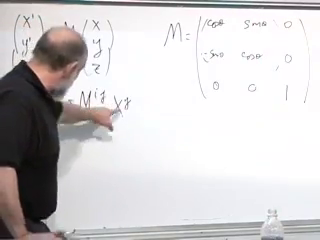
\includegraphics[width=0.82\textwidth]{lecture_05_figure_03.png}
\caption{Пространственный поворот, записанный и как матричное уравнение, и в индексной форме.}
\lectureframe{01:00:40}
\end{figure}

\section{Матрицы Лоренца и сложение скоростей}

Для движения вдоль \(x\) лоренцево преобразование в единицах \(c=1\) имеет вид
\begin{align}
x'&=\gamma_v(x-vt), & y'&=y,\nonumber\\
z'&=z, & t'&=\gamma_v(t-vx),
\end{align}
где
\begin{equation}
\gamma_v=\frac{1}{\sqrt{1-v^2}}.
\end{equation}
При порядке компонент \((x,y,z,t)\) это принимает вид
\begin{equation}
\begin{pmatrix}x'\\y'\\z'\\t'\end{pmatrix}
=
\begin{pmatrix}
\gamma_v&0&0&-\gamma_vv\\
0&1&0&0\\
0&0&1&0\\
-\gamma_vv&0&0&\gamma_v
\end{pmatrix}
\begin{pmatrix}x\\y\\z\\t\end{pmatrix}.
\label{eq:l5-lorentz-matrix}
\end{equation}

\begin{figure}[H]
\centering
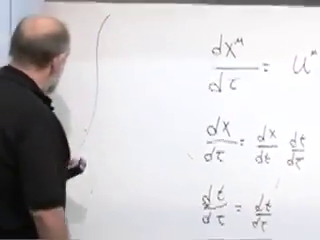
\includegraphics[width=0.82\textwidth]{lecture_05_figure_04.png}
\caption{Матрица Лоренца \(4\times4\). Смешиваются только компоненты \(x\) и \(t\); \(y\) и \(z\) остаются неизменными.}
\lectureframe{01:04:40}
\end{figure}

Теперь матричное умножение позволяет ответить на физический вопрос. Предположим, что один наблюдатель движется со скоростью \(v\) относительно нас, а третий — со скоростью \(u\) относительно него, причём все движутся вдоль одной и той же оси. Ньютоновская кинематика дала бы \(w=u+v\), что позволяло бы двум скоростям по \(3c/4\) сложиться в \(3c/2\). Теория относительности должна давать другое правило.

Нетривиальная часть буста — это матрица \(2\times2\)
\begin{equation}
B(v)=\gamma_v
\begin{pmatrix}1&-v\\-v&1\end{pmatrix}.
\end{equation}
Композиция двух бустов даёт
\begin{align}
B(u)B(v)
&=\gamma_u\gamma_v
\begin{pmatrix}1&-u\\-u&1\end{pmatrix}
\begin{pmatrix}1&-v\\-v&1\end{pmatrix}\nonumber\\
&=\gamma_u\gamma_v
\begin{pmatrix}
1+uv&-(u+v)\\
-(u+v)&1+uv
\end{pmatrix}.
\label{eq:l5-composed-boost}
\end{align}
Отношение внедиагонального элемента к диагональному определяет скорость результирующего буста:
\begin{equation}
w=\frac{u+v}{1+uv}
\qquad(c=1).
\end{equation}
Восстанавливая размерности,
\begin{equation}
w=\frac{u+v}{1+uv/c^2}.
\label{eq:l5-velocity-addition}
\end{equation}

\begin{figure}[H]
\centering
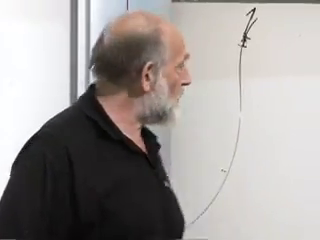
\includegraphics[width=0.82\textwidth]{lecture_05_figure_05.png}
\caption{Матрица композиции бустов и скорость
\(w=(u+v)/(1+uv)\) в естественных единицах.}
\lectureframe{01:15:35}
\end{figure}

Если \(u\) и \(v\) каждая близка к \(c\), числитель стремится к \(2c\), а знаменатель — к \(2\), так что \(w\) стремится к \(c\), а не к \(2c\). В более общем виде Eq.~\eqref{eq:l5-velocity-addition} отображает досветовые значения в досветовой результат. Матричное умножение автоматически закодировало предел скорости.

\section{Четырёхвекторы и непригодность обычной скорости}

Четырёхвектор — это любой объект, четыре компоненты которого преобразуются при поворотах и бустах Лоренца так же, как координаты пространства-времени. Если \(V^\mu\) — четырёхвектор, то при нашем соглашении о знаках
\begin{equation}
V_\mu=(-V^1,-V^2,-V^3,V^0),
\end{equation}
а его инвариантная норма равна
\begin{equation}
V_\mu V^\mu=(V^0)^2-(V^1)^2-(V^2)^2-(V^3)^2.
\end{equation}
Для двух четырёхвекторов \(V^\mu\) и \(W^\mu\) свёртка
\begin{equation}
W_\mu V^\mu
=W^0V^0-W^1V^1-W^2V^2-W^3V^3
\end{equation}
также инвариантна. Компоненты меняются при переходе от одной системы отсчёта к другой; свёртка — нет.

Обычная скорость имеет только три компоненты,
\begin{equation}
\mathbf v=\left(\frac{dx}{dt},\frac{dy}{dt},\frac{dz}{dt}\right).
\end{equation}
Добавление \(dt/dt=1\) не делает из неё полезный четырёхвектор. Четвёртая компонента была бы тривиальной, и получившийся объект не преобразовывался бы линейно при преобразованиях Лоренца. Координатное время \(t\) меняется от одной системы отсчёта к другой, поэтому дифференцирование по \(t\) нарушает требуемый закон преобразования.

Собственное время решает эту проблему. Вдоль мировой линии определим
\begin{equation}
u^\mu=\frac{dX^\mu}{d\tau}.
\label{eq:l5-four-velocity}
\end{equation}
Дифференциал \(dX^\mu\) является четырёхвектором, а величина \(d\tau\) инвариантна, поэтому их отношение — четырёхвектор. Прилагательное ``собственный'' относится к часам в знаменателе.

Правило цепочки связывает эту величину с обычной скоростью:
\begin{equation}
\frac{dx}{d\tau}=\frac{dx}{dt}\frac{dt}{d\tau},
\end{equation}
и аналогично для \(y\) и \(z\). Из уравнения~\eqref{eq:l5-proper-time},
\begin{align}
\left(\frac{d\tau}{dt}\right)^2
&=1-\left(\frac{dx}{dt}\right)^2
    -\left(\frac{dy}{dt}\right)^2
    -\left(\frac{dz}{dt}\right)^2\nonumber\\
&=1-v^2
\qquad(c=1),
\end{align}
и поэтому
\begin{equation}
\frac{dt}{d\tau}=\gamma_v=\frac{1}{\sqrt{1-v^2}}.
\end{equation}
Четыре компоненты имеют вид
\begin{equation}
u^i=\gamma_v v^i,
\qquad
u^0=\gamma_v
\qquad(c=1).
\label{eq:l5-four-velocity-components}
\end{equation}
При малой скорости \(u^i\simeq v^i\) и \(u^0\simeq1\). При скоростях, близких к скорости света,
\(\gamma_v\) неограниченно возрастает, и собственная скорость резко отличается от обычной.

\begin{figure}[H]
\centering
\includegraphics[width=0.82\textwidth]{lecture_05_figure_06.png}
\caption{Четыре компоненты собственной скорости, выраженные через обычную скорость и фактор Лоренца.}
\lectureframe{01:34:40}
\end{figure}

Восстанавливая обычные единицы и используя \(X^0=ct\), получаем стандартный вид
\begin{equation}
U^\mu=(\gamma_v\mathbf v,\gamma_v c)
\end{equation}
в используемом здесь порядке, где пространственные компоненты стоят первыми. Его инвариантная норма равна
\begin{equation}
U_\mu U^\mu=c^2.
\end{equation}
Следовательно, у любой массивной частицы модуль четырёхскорости имеет одно и то же инвариантное значение, хотя её пространственная скорость зависит от системы отсчёта.

\section{Касательный вектор к мировой линии}

Для уравнения~\eqref{eq:l5-four-velocity} есть знакомая евклидова модель. Вдоль кривой в обычном трёхмерном пространстве,
\begin{equation}
ds^2=dx^2+dy^2+dz^2.
\end{equation}
Дифференциальное смещение \((dx,dy,dz)\) направлено вдоль кривой, но не является единичным вектором. Деление на длину дуги даёт
\begin{equation}
\mathbf T=
\left(\frac{dx}{ds},\frac{dy}{ds},\frac{dz}{ds}\right),
\qquad
\mathbf T\cdot\mathbf T=1.
\end{equation}
Релятивистская конструкция — это та же идея, только с собственным временем вместо евклидовой длины дуги. Вектор \(u^\mu=dX^\mu/d\tau\) является касательным к мировой линии.

\begin{figure}[H]
\centering
\includegraphics[width=0.82\textwidth]{lecture_05_figure_07.png}
\caption{Евклидова конструкция касательного вектора: дифференциальное смещение делится на элемент длины дуги \(ds\). Собственное время играет аналогичную роль вдоль времеподобной мировой линии.}
\lectureframe{01:39:30}
\end{figure}

\begin{classroomqa}
\audiencequestion{Если \(c=1\), то собственное время и собственное расстояние — одно и то же?}
\lecturerresponse{Положив \(c=1\), мы выражаем время и расстояние в одних и тех же единицах; это не устраняет знаки минус в геометрии пространства-времени. В евклидовой аналогии \(s\) — это обычное расстояние, измеряемое вдоль пространственной кривой. Вдоль времеподобной мировой линии \(\tau\) — это прошедшее время, измеряемое часами. Конструкции аналогичны, но геометрии различны.}
\end{classroomqa}

Ещё одно дифференцирование определяет собственное ускорение,
\begin{equation}
a^\mu=\frac{du^\mu}{d\tau}.
\end{equation}
Именно эта величина должна заменить \(d^2\mathbf x/dt^2\), когда второму закону Ньютона придают релятивистскую форму. Поскольку величина \(u_\mu u^\mu\) постоянна,
\begin{equation}
\frac{d}{d\tau}(u_\mu u^\mu)=2u_\mu a^\mu=0,
\end{equation}
так что четырёхускорение ортогонально четырёхскорости относительно метрики Минковского.\editorialnote{Ортогональность немедленно следует из инвариантной нормы и включена как следующее математическое следствие определения.}

\section{Четырёхимпульс и энергия}

Импульс — наш последний пример, потому что он сохраняется при столкновениях и распадах. У частицы есть фиксированная присущая ей масса \(m\), которую часто называют массой покоя. Она не зависит от скорости. Релятивистский импульс равен произведению этой фиксированной массы на четырёхскорость:
\begin{equation}
p^\mu=mu^\mu.
\label{eq:l5-four-momentum}
\end{equation}
В единицах \(c=1\),
\begin{equation}
p^i=\gamma_v m v^i,
\qquad
p^0=\gamma_v m.
\end{equation}
При малой скорости \(\gamma_v\simeq1\), поэтому пространственные компоненты сводятся к ньютоновскому импульсу \(m\mathbf v\). При большой скорости они растут быстрее, чем \(m\mathbf v\).

Временная компонента — это энергия. В обычных единицах и при \(X^0=ct\),
\begin{equation}
P^\mu=(\mathbf p,E/c)
=(\gamma_v m\mathbf v,\gamma_v mc),
\end{equation}
и, следовательно,
\begin{equation}
E=\gamma_v mc^2
=mc^2\left(1-\frac{v^2}{c^2}\right)^{-1/2}.
\label{eq:l5-relativistic-energy}
\end{equation}

Чтобы вернуться к обычной механике, положим
\(\epsilon=v^2/c^2\ll1\). Биномиальное разложение даёт
\begin{equation}
(1-\epsilon)^p=1-p\epsilon+O(\epsilon^2).
\end{equation}
Подставляя \(p=-1/2\),
\begin{align}
E
&=mc^2\left(1-\frac{v^2}{c^2}\right)^{-1/2}\nonumber\\
&=mc^2\left[1+\frac12\frac{v^2}{c^2}
  +O\!\left(\frac{v^4}{c^4}\right)\right]\nonumber\\
&=mc^2+\frac12mv^2+O\!\left(\frac{mv^4}{c^2}\right).
\label{eq:l5-energy-expansion}
\end{align}

\begin{figure}[H]
\centering
\includegraphics[width=0.82\textwidth]{lecture_05_figure_08.png}
\caption{Разложение релятивистской энергии по малой скорости, выявляющее энергию покоя и ньютоновскую кинетическую энергию.}
\lectureframe{01:51:30}
\end{figure}

Первый член, \(mc^2\), присутствует даже в покое. В ньютоновской задаче с фиксированным набором частиц и неизменными массами этот член добавляет одну и ту же константу до и после движения, поэтому для привычного учёта имеет значение только \(\tfrac12mv^2\). Теория относительности показывает, что отброшенная константа всё это время была физической энергией.

Следовательно, энергия и импульс — не два несвязанных закона сохранения. Они являются четырьмя компонентами одного сохраняющегося вектора. Буст Лоренца смешивает их: то, что один наблюдатель называет энергией, частично входит в импульс другого наблюдателя, и наоборот. Тем не менее для изолированной системы полный четырёхимпульс одинаков до и после каждого столкновения или распада в любой инерциальной системе отсчёта.

Это порог релятивистской механики. Следующие задачи — выразить силу через собственное ускорение и понять релятивистские волновые уравнения, особенно уравнения, описывающие электромагнетизм и свет.
